%%%%%%%%%%%%%%%%%%%%%%%%%%%%%%%%%%%%%%%%%%%%%%%%%%%%%%%%%%%%%%%%%%%%%%%% 
%%%%%%%%%%%%%%%%%%%%%%%%%%%%%%%%%%%%%%%%%%%%%%%%%%%%%%%%%%%%%%%%%%%%%%%% 
\begin{frame}[fragile=singleslide]
  \frametitle{Hands-On 6 : Random number generator with Kokkos}

  \begin{itemize}
  \item Activity: \textcolor{red}{\bf Estimating Pi via Monte Carlo}
  \item purpose: learn to use the {\bf random number generator} features (built-in Kokkos)
  \item Draw random points in $[0,1]^2$ and compute the fraction of points inside the unit circle:
    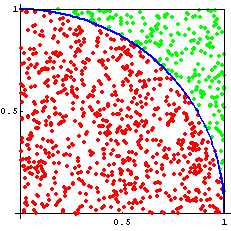
\includegraphics[width=2.5cm]{images/MonteCarloPiMod_gr_25}
  \item These generators are based on Vigna, Sebastiano (2014). {\it An experimental exploration of Marsaglia's xorshift generators, scrambled.} \myurl{http://arxiv.org/abs/1402.6246}
  \item Use code in \texttt{code/handson/6/compute\_pi}; read \texttt{readme} file; fill the holes
  \item Which compute pattern will you use ? \texttt{parallel\_for}, \texttt{parallel\_reduce}, \texttt{parallel\_scan} ?
  \end{itemize}
  
\end{frame}

%%%%%%%%%%%%%%%%%%%%%%%%%%%%%%%%%%%%%%%%%%%%%%%%%%%%%%%%%%%%%%%%%%%%%%%% 
%%%%%%%%%%%%%%%%%%%%%%%%%%%%%%%%%%%%%%%%%%%%%%%%%%%%%%%%%%%%%%%%%%%%%%%% 
\begin{frame}[fragile=singleslide]
  \frametitle{Hands-On 6 : Random number generator with Kokkos}

  {\bf \large Random number generator in Kokkos: the big picture}
  \begin{itemize}
  \item Kokkos defines tuple of types (\textcolor{red}{RNG state}, \textcolor{blue}{RNG pool})\\
    e.g. (\texttt{Random\_XorShift64}, \texttt{Random\_XorShift64\_Pool})
  \item Kokkos defines several type of random generator, the main object is a \textcolor{blue}{\bf random number generator pool} of \textcolor{red}{\it RNG states}, e.g. \textcolor{blue}{\bf \texttt{Kokkos::Random\_XorShift64\_Pool}}
    \begin{itemize}
    \item this is a template class, which takes a Kokkos device as template parameter (Kokkos::OpenMP, Kokkos::Cuda, ...)
    \item the pool constructor takes an integral seed to initialize, (option) the number of states in pool
    \item it is basically an array of {\it RNG states}
    \end{itemize}
  \item A random generator pool defines a subtype to store a given random generator \textcolor{red}{\bf internal state}: so that inside a functor, one would find:\\
    \texttt{using rng\_state\_t = GeneratorPool::generator\_type}
  \item rule of thumb:\\
    One pool $\Leftrightarrow$ one functor\\
    One rng\_state $\Leftrightarrow$ (use by) one thread
  \end{itemize}
\end{frame}

%%%%%%%%%%%%%%%%%%%%%%%%%%%%%%%%%%%%%%%%%%%%%%%%%%%%%%%%%%%%%%%%%%%%%%%% 
%%%%%%%%%%%%%%%%%%%%%%%%%%%%%%%%%%%%%%%%%%%%%%%%%%%%%%%%%%%%%%%%%%%%%%%% 
\begin{frame}[fragile=singleslide]
  \frametitle{Hands-On 6 : Random number generator with Kokkos}

  \textcolor{blue}{\bf \large RNG pool interface}\\
  get / release a RNG state from the pool in a kokkos thread
  \begin{minted}{c++}
    template<class DeviceType = Kokkos::DefaultExecutionSpace>
    class Random_XorShift64_Pool {
      private:
      int num_states_;
      // ...
      public:
      Random_XorShift64_Pool(uint64_t seed) {...}

      KOKKOS_INLINE_FUNCTION
      Random_XorShift64<DeviceType> get_state() const {...}

      KOKKOS_INLINE_FUNCTION
      void free_state(const Random_XorShift64<DeviceType>& state) const {...}
    };
  \end{minted}

\end{frame}

%%%%%%%%%%%%%%%%%%%%%%%%%%%%%%%%%%%%%%%%%%%%%%%%%%%%%%%%%%%%%%%%%%%%%%%% 
%%%%%%%%%%%%%%%%%%%%%%%%%%%%%%%%%%%%%%%%%%%%%%%%%%%%%%%%%%%%%%%%%%%%%%%% 
\begin{frame}[fragile=singleslide]
  \frametitle{Hands-On 6 : Random number generator with Kokkos}

  \textcolor{red}{\bf \large RNG state interface}
  \begin{minted}{c++}
    template<class DeviceType>
    class Random_XorShift64 {
      private:
      // state variables...
      public:

      // multiple inline methods to return a rand number
      KOKKOS_INLINE_FUNCTION
      int rand() {
        return ... ;
      }
    };
  \end{minted}

\end{frame}

%%%%%%%%%%%%%%%%%%%%%%%%%%%%%%%%%%%%%%%%%%%%%%%%%%%%%%%%%%%%%%%%%%%%%%%% 
%%%%%%%%%%%%%%%%%%%%%%%%%%%%%%%%%%%%%%%%%%%%%%%%%%%%%%%%%%%%%%%%%%%%%%%% 
\begin{frame}[fragile=singleslide]
  \frametitle{Hands-On 6 : Random number generator with Kokkos}

  \textcolor{orange}{\bf \large \texttt{struct rand} interface}
  \begin{itemize}
  \item A wrap-up / helper class to draw random numbers with uniform law (static method \texttt{draw}):
    \begin{minted}{c++}
      template<class Generator,Scalar>
      struct rand {
        //Returns a value between zero and max()
        KOKKOS_INLINE_FUNCTION
        static Scalar draw(Generator& gen);
      };
    \end{minted}
  \item {\bf How to use RNG in a user application ?}
    \begin{itemize}
    \item the driving code create a \textcolor{blue}{\bf RNG pool}, and pass it to a functor constructor.
    \item Inside a kokkos kernel functor, a thread must retrieve a \textcolor{red}{\bf RNG state} from the pool, \textcolor{orange}{\bf draw some random numbers}, release the \textcolor{red}{\bf RNG state}.
    \end{itemize}
  \end{itemize}
  
  \textcolor{darkgreen}{\bf \large Exercise:}
  \begin{itemize}
  \item open file \texttt{src/compute\_pi.cpp}; \textcolor{darkgreen}{\bf try to fill the holes (at location of TODO)}
  \item Explore the OpenMP and Cuda version efficiency
  \end{itemize}
  
\end{frame}